\documentclass[a4paper]{article}
\usepackage{amsmath}
\usepackage{amsfonts}
\usepackage{amsthm}
\usepackage{amssymb}
\usepackage[english]{babel}
\usepackage{float}
\usepackage{graphicx}
\usepackage{hyperref}
\usepackage[utf8]{inputenc}
\usepackage{listings}
\usepackage{xcolor}
%% \usepackage{subfigure}
\usepackage{pdfpages}
\usepackage{graphicx}
\usepackage{subcaption}
\usepackage{stmaryrd}
\usepackage{a4wide}

\lstset{
  frame=tb,
  language=Python,
  aboveskip=3mm,
  belowskip=3mm,
  showstringspaces=false,
  formfeed=newpage,
  tabsize=4,
  comment=[l]{\#},
  breaklines=true,
  basicstyle=\small
}

\newcommand{\prob}[1]{\mathbb{P}\left(#1\right)}
\newcommand{\expect}[1]{\mathbb{E}\left(#1\right)}
\newcommand{\avg}[1]{\sum_{i=1}^{#1}X_i}
%% \newcommand{\dotp}[2]{\langle #1 + #2 \rangle}
%% \newcommand{\dotp}[2]{\ensuremath{\frac{#1}{#2}}}
\newcommand{\dotpr}[2]{\langle #1,\; #2 \rangle}
\newcommand{\norm}[1]{\left\lVert#1\right\rVert}
\newcommand*{\QEDA}{\hfill\ensuremath{\blacksquare}}%

\title{\vspace{-5cm}ATML Home Assignment 3}
\author{Dmitry Serykh (qwl888)}

\begin{document}
\maketitle
\section{Description}
\subsection{Practical Information}
In this assignment, I have attempted to reproduce the second experiment from
Thiemann et al for the Ionosphere dataset. I based a portion of my implementation
(including the calculation Jaakkola's heuristic) on my own solution to a similar
exercise from the ML course. I used \emph{python}, \emph{numpy} and SVM solver
from the \emph{sklearn} package. The experiment were ran on my laptop, running
Linux and with following hardware specifications:
\begin{verbatim}
 CPU: Intel Core i7-3520M @ 4x 3.6GHz
 RAM: 7682MiB
\end{verbatim}

\subsection{Theory}
I used the slightly tighter version of PAC-Bayes-kl inequality, as described in
the assignment. Furthermore, I used a following numerically stable update rule for $\rho$,
as suggested in the assignment text.
\[
\rho(h) = 
\frac{\left.\pi(h) e^{-\lambda(n-r)\left(\hat{L}^{\mathrm{val}(h, S)}-\hat{L}_{\mathrm{min}}^{\mathrm{val}}\right.}\right)}{\sum_{h^{\prime}} \pi\left(h^{\prime}\right) e^{-\lambda(n-r)\left(\hat{L}^{\mathrm{val}}\left(h^{\prime}, S\right)-\hat{L}_{\mathrm{min}}^{\mathrm{val}}\right)}}
\]

\subsection{Results}
I decided to not repeat the ``sin'', committed in the original paper and
repeated the whole experiment 25 times and found the average of the gathered
results. Moreover, I calculated the standard deviation of the losses and
runtimes for both methods:

\begin{verbatim}
Standard deviations:
PAC Bayes loss: 0.0982
CV loss: 0.0147
PAC Bayes time: 0.0575
CV time: 0.0441
\end{verbatim}
The resulting plot of average test losses,
running time and bound can be seen on Figure \ref{plt1}. The source code for my
implementation can be found in file \texttt{experiment.py} in
\textbf{handin.zip}.

\section{Conclusion}
I reproduced the experiment from the paper and managed to achieve a similar
looking result. The values of test loss are closer to the baseline model when
the value of $m$ approaches $n$, as in the paper. Furthermore, the runtime
for the method, used in the paper is much better than the baseline model. The
difference is very similar to the experiment in the paper.
As one would expect, there are differences between the plots due
to random nature of the algorithm.

\begin{figure}
  \centering
  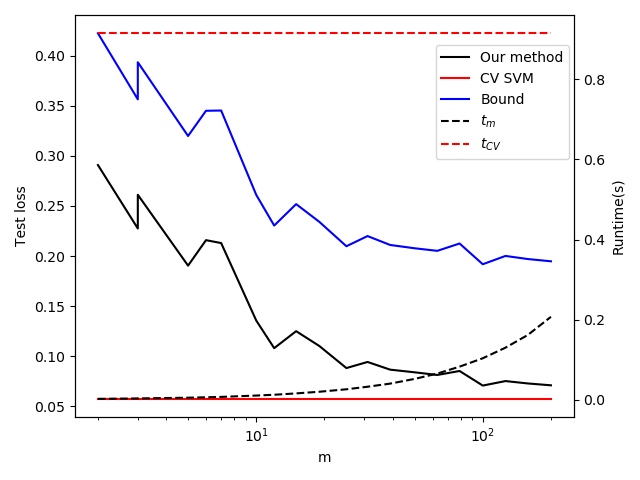
\includegraphics[width=\textwidth]{code/plt_avg25}
  \caption{Comparison of PAC-Bayesian aggregation with RBF kernel SVM
    tuned by cross-validation for the Ionosphere dataset. Averaged over 25 experiments, $n=200$, $r=35$}
  \label{plt1}
\end{figure}

\end{document}

%% \begin{figure}
%%   \centering
%%   \begin{subfigure}[b]{\textwidth}
%%     \centering
%%     \includegraphics[scale=0.8]{handin/plt51}
%%     \caption{Classification of the training set}
%%   \end{subfigure}
%%   \begin{subfigure}[b]{\textwidth}
%%     \centering
%%     \includegraphics[scale=0.8]{handin/plt52}
%%     \caption{Classification of the test set}
%%   \end{subfigure}
%%   \caption{Exercise 5: Logistic Regression Applied to the Datasets}
%%   \label{plt5}
%% \end{figure}

%% \begin{lstlisting}[caption="Calculation of g"]
%% def calc_g(Xs, y, w):
%%     N = np.shape(Xs)[0]
%%     # use matrix X of xs instead of for-loop = much faster
%%     X = np.c_[Xs, np.ones(N)]
%%     num = y.T * X
%%     denum = 1 + np.exp(y * (w @ X.T))
%%     M = num.T/denum
%%     # return mean of each row
%%     return (-1 * np.mean(M, axis=1))
%% \end{lstlisting}
